\chapter{提案手法}
\label{chapter:proposal}
データセンターにおけるマルチパスネットワークの研究動向と, 並列分散処理アプリケーションが生成する特有のトラフィックパターンが引き起こす機能障害をふまえて,
改善手法を提案する.
本提案手法では, 
汎用的なネットワーク機器で構成されたデータセンターネットワークにおいて, エンドノードのみの改良によって, 
バースト性のあるトラフィックが通信している中でのサイズ小さいフロー通信に対するスケーラビリティと低遅延を達成することを目指す.
この目的を達成するために, 提案手法では指向が異なるフローを区別する制御を行い,
スループット指向なフローについては複数の経路を用いてスループットを向上し, レイテンシ指向なフローについてキューイング遅延を小さくする通信を行う.

\section{Motivation}
提案手法の動機となったのは, MPTCPを用いたデータセンターネットワークモデルである\cite{improving}.
今日のデータセンターネットワークは, FatTreeトポロジーやClosトポロジーに基づいた構成になっており\cite{dctcp, vl2},
複数の等しいコストの経路が存在している. 
提案されたネットワークモデルでは, エンドノードが複数のNICを持ち,
MPTCPによって一つのフローの通信で複数の経路を同時に利用することでスループットを向上させる.
このような複数経路の効率的利用には, IPベースのルーティングで実現しており, それぞれのエンドノードが持つIPアドレスのペアにより, 通信経路が決定する.
現在のMPTCPの実装では, TCPコネクション確立後に互いのIPアドレスを交換し,
新しいサブフローを形成する仕組みになっており, サイズの小さいフローの通信では, サブフローが形成されないまま通信が完結する問題がある. 
その結果, 一つの経路に通信が集中することで中継スイッチのキューが圧迫され, フローの遅延が大きくなる. 
実際, 以前の我々の解析でも, このコネクション確立の際に遅延が生じることが分かっており\cite{mptcp_ana}, どの経路を利用するかによって,
性能性能が大きく変わる.

複数経路の有効活用の手法として, ECMPによるフロー単位でのルーティングがある. 
ECMPではパケットヘッダーの5タプルを用いたハッシュベースのルーティングやラウンドロビンによって, ランダムに経路を選択し, 負荷分散していく. 
この不完全なランダム性のために, ショートフローとロングフローが同一の経路に振り分けられることが起こり,
ショートフローはFCFS(First-Come-First-Serve)方式のキューシステムによって, キューイング遅延が発生する. 
今, Fig.\ref{fig:repflow_scenario}のようなネットワークシナリオを考える. 
このトポロジーは$k=4$ FatTreeトポロジーでのある1ポッド内での通信を示している. 
スイッチS1(S2)と接続されている二つのノードともう一方のノード間にはと二つの等しいコストの経路があり, H2からH4に対してS1-S3-S2の経路を通り,
ロングフローが通信している状況を考える. 
今, H1はH3に対してショートフロー通信を行おうとしたとき, ECMPによるランダムルーティングにより,
$0.5$の確率で同じ経路S1-S3-S2を選択してしまう. 
その結果, ロングフローによってキューイング遅延の影響を受ける. 
実際, $\S$\ref{sec:verification}に示すように実機を用いてこの同一経路を通る問題を検証したところ,
ロングフローをうまく負荷分散した時と同一の経路で通信した時の95パーセンタイル値FCTにおいて,
約10倍程度性能が劣化することがわかった\cite{mptcp_ana2}.
そのため, ロングフローはS1-S3-S2の経路を通り, ショートフローはS1-S4-S2の経路を通るように, 分散させて通信することが,
マルチパス環境における複数経路の効率的な利用の理想的な状況である. 

\begin{figure}[t]
    \begin{center}
    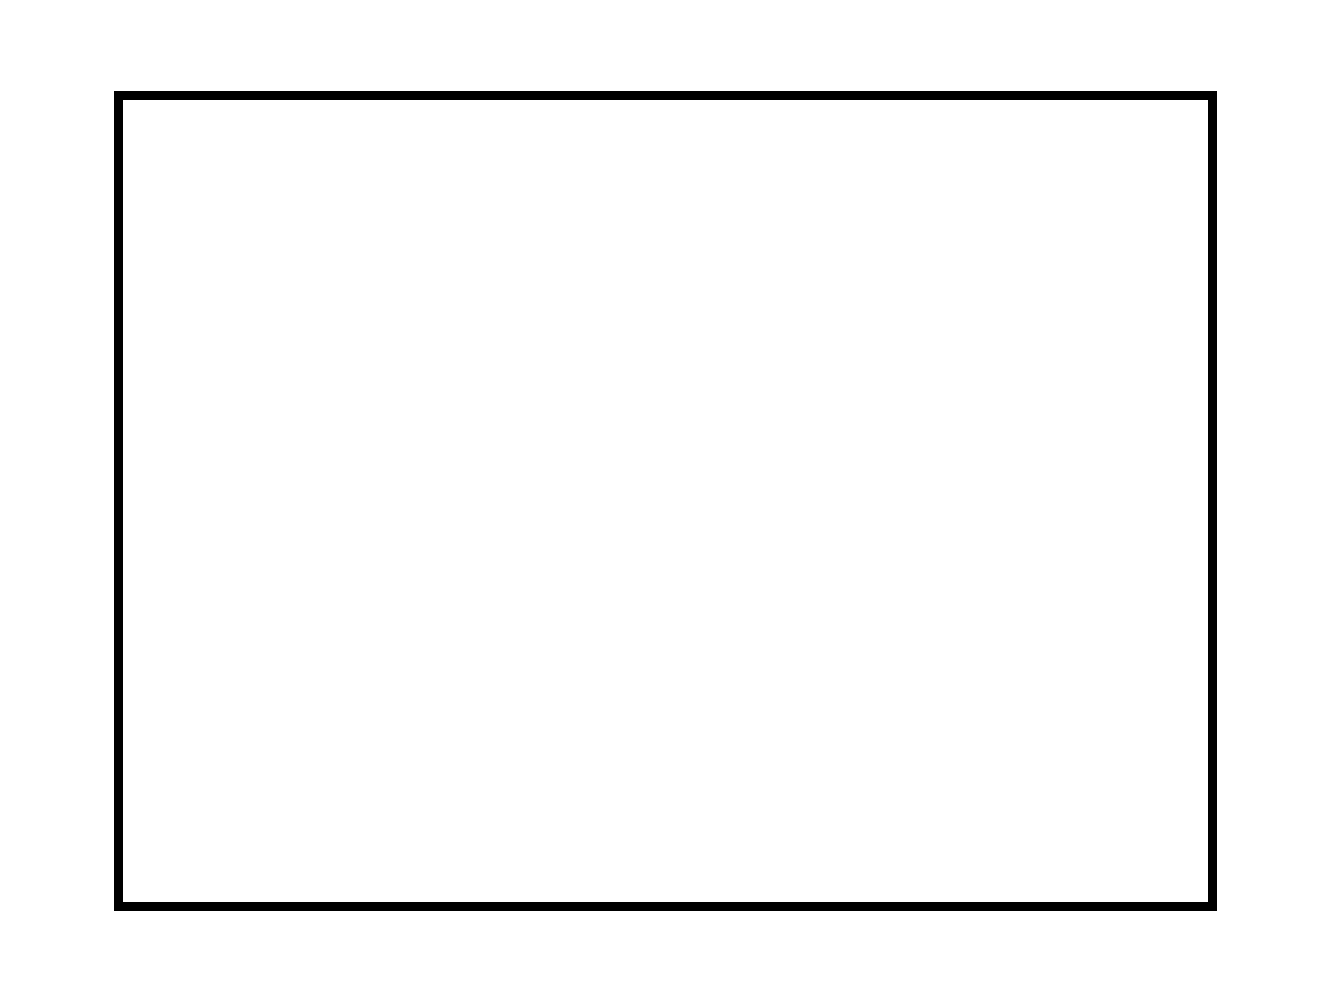
\includegraphics[autoebb, width=200pt]{./img/test.pdf}
    \caption{Scenario of queue buildup problem with multi-cost paths)}
    %\ecaption{The control loop in DCTCP}
    \label{fig:repflow_scenario}
    \end{center}
\end{figure}


\section{本研究の位置付け}
\label{sec:myworks_position}
$\S$\ref{chapter:related_work}に示した既存研究のように, 
データセンターネットワークでのショートフロー問題を解決する取り組みはされており, その中で本研究手法の位置付けを以下に示す. 
\begin{enumerate}
\item スイッチに対して特殊な実装を施さないこと. 
\item 既存のアプリケーションにも変更なく使えるようにすること. 
\item ショートフローのFCTだけでなく, ロングフローのスループットについても改善すること. 
\end{enumerate} 

1. については, $\S$\ref{chapter:related_work}に示した多くの手法がスイッチに対して変更を加え,
キューイング遅延が起こっている箇所から直接情報を得てエンドノードに通達する. 
しかし, スイッチに対して実装や変更を加えることで, 全てのスイッチに対してそれらを行う必要性があるため, 実環境への適用に問題があると言える. 
実際, 様々な種類のネットワーク機器が混在している中ではなおさら実現困難である\cite{d3}.

2. については, RepFlowは中継スイッチに変更を必要とせず, エンドノード間の変更のみで改善することができる手法であるが, 現状の実装だと,
アプリケーションに対する変更が必要であるため, 既存のアプリケーションに対して適用しようとした場合,
それらに対して変更が必要である\cite{repflow}.
そのため, 実現可能性の観点では有効手法であるとは言えない. 

3. については, $\S$\ref{sec:verification}に示すように, ロングフローとショートフローが同一の経路で通信を行った場合, 
このように, ECMPによる負荷分散手法では深刻な遅延の問題を引き起こすこととなる. 
$\S$\ref{sec:verification}に示す検証実験では, ショートフローの性能劣化だけでなく,
ロングフローのスループットについても約30\%程度利用率が劣化する結果が得られた. 
RepFlowでは, ショートフローに対して同一の通信を複製することによって, キューイング遅延のない経路を通る,
ショートフローに対して最小のFCTを達成できるという手法であるが, 複製の結果, ロングフローのスループット性能も劣化することが考えられる. 
%そのため, レイテンシ指向なショートフローと, スループット指向なロングフローのように区別して

以上を踏まえて本研究における位置付けを以下のように設定する. 
\begin{enumerate}
\item エンドノード間のみのアプローチでこれを解決する. 
\item OSのみに変更を加え, 既存のアプリケーションに変更を加えず適用できる. 
\item フローを指向ごとに区別し, それぞれに応じた改善を行うこと. 
\end{enumerate} 

Fig.\ref{fig:repflow_scenario}の場合, 実環境においては,
エンドノード間のみの通信で, ショートフローが前もって正しい経路を選択するためには,
事前に輻輳検出用のトラフィックによって通信状況を取得する手法がなされているが, 十分な検出精度を得るためのサンプリング時間のために,
通信オーバーヘッドの影響がある\cite{devoflow}.
そのため本研究では, データセンターネットワーク内に指向毎にレーンを設けるデータセンターレーンモデルと, その指向を区別し,
それぞれの経路を切り替えるためのアルゴリズムを提案する. 

\section{Design}

\subsection{データセンターレーンモデル}
\label{subsec:lane_model}
本小節では, 指向毎にフローを切り替えて制御するためのネットワークモデルとして, データセンターレーンモデルを示し,
そのトポロジーと動作するアーキテクチャについて詳しく示す. 

\subsubsection{BackGround}

今日のネットワーク機器において, コモディティ化し安価な機器と, ある用途に特化した高価な機器のコストの差は明確となっており,
データセンター事業者はその性能とコストのトレードオフについて考慮しなければならず,
なるべくコストを抑えたい要求に対して頭を悩ませている\cite{fattree}.
50年以上前の電話網の形成の際にも, 多くの汎用的なスイッチを用いてより多くの端末に接続できるような設計が行われた\cite{clos}. 
そうしたClosトポロジーに基づき,
Ethernetスイッチによって構成されるネットワークトポロジーの一つにFatTreeトポロジーがある\cite{fattree}. 

Full-bisectionalトポロジーに対する, 要求案件として以下のようなものが考えられる\cite{improving}.
\begin{itemize}
\item 局所性のないトラフィック
\item すべてのホストが最大帯域活用できる
\item どのアクセスリンクに対してもトラフィックの集中がない
\end{itemize} 
%実際にはこれらの案件が同時に必要となる場合は起こり得ないと考えられ,
%Full-bisectionalな帯域を提供することはコストの面から最適であるとは言いにくい.

今FatTreeトポロジーに対して, 並列分散処理システムを適用させることを考え, HDFSによって同じラックの異なるホストにデータを複製し,
MapReduceによるmapタスクがそれらに対して割り当てられるとする.
つまり, 同一ポッド内でのトラフィックが発生する.
MPTCPは基本的にコアに対するトラフィックに対して有効に働くが, このようなローカルなトラフィックに対して, 十分に機能しない. 

もしすべてのノードに対してMPTCPが実装されたとき, よりMPTCPの特性を引き出すようなトポロジーを検討する必要がある. 
具体的には, エンドノードとToR(Top-of-Rack)スイッチ間のアクセスリンクでボトルネックが発生した時, 効率的な帯域の利用を考える. 
例えば, 1GEthernetリンクから10Gリンクへと変更することでより広帯域なネットワークを実現できるが, コスト面の問題がある. 
また, 従来のSigle-path TCPでは, 1本のリンク容量以上の帯域を得ることはできないという制限がある. 
しかしMPTCPでは, そのような制限はない. 
実際, 近年のサーバ機器には基本的に複数のギガビットイーサネットインタフェースが搭載されており, エンドノードが二つのNICを持つ際のトポロジーとして,
DHFT(Dual-Homing FatTree)トポロジーが提案されている. 
そこで本研究ではDHFTを発展させた複数NICを用いたMHFT(Multi-Homing FatTree)トポロジーを提案し,
MPTCPによる効率的な帯域利用を実現する. 

\subsubsection{トポロジー}
Fig.\ref{fig:multi-homing}に提案するk-ary MHFTを示す. 
k-aryマルチホーミングトポロジーはFatTreeと同様に, k個のポッドから構成されおり, 
一つのポッドで$k/2, k^2/4$それぞれaggregatorスイッチとedgeスイッチを持つ. 
aggregatorスイッチとedgeスイッチではそれぞれ,
$k/2$のノードと上位レイヤーのスイッチ1つに接続し, 計$k/2+1$ポートが必要である. 
また, coreスイッチは$k/2$台の$k/2$ポートスイッチが必要である. 
また, MHFTは$k^3/4$までのノードを持つことができる. 

\begin{figure}[t]
    \begin{center}
    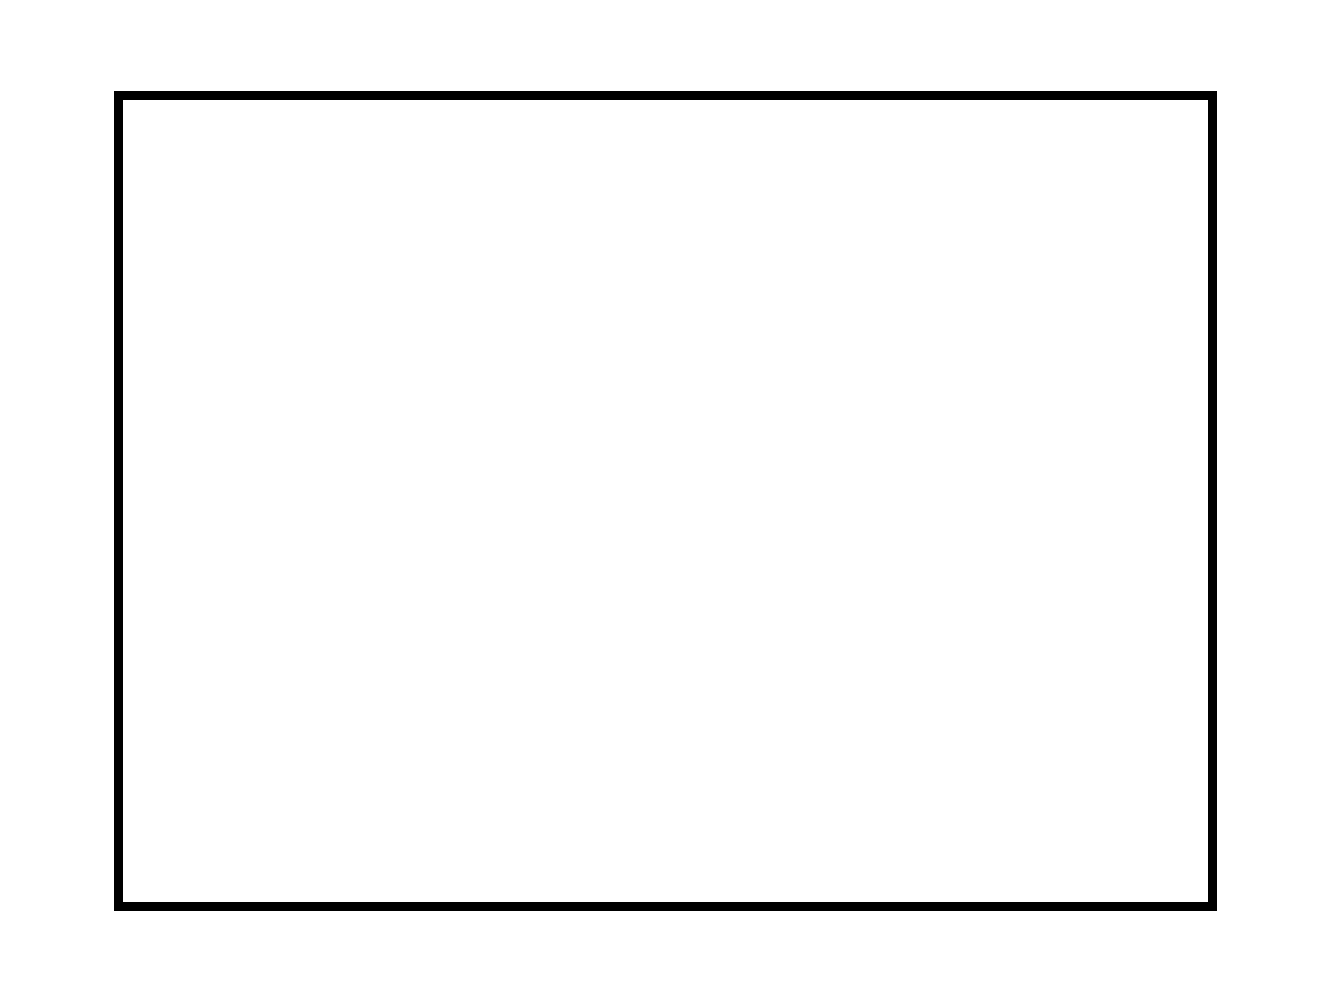
\includegraphics[autoebb, width=200pt]{./img/test.pdf}
    \caption{Multi-homing in the FatTree Topology}
    %\ecaption{The control loop in DCTCP}
    \label{fig:multi-homing}
    \end{center}
\end{figure}

\begin{table}[t]
    \begin{center}
    \begin{tabular}{|c|c|c|}
    \hline
    k-ary & Number & Port/Interface \\ \hline \hline
    core & $k/2$ & $k/2$ \\ \hline
    aggregator & $k^2/2$ & $k / 2 + 1$ \\ \hline
    edge & $k^3 / 4$ & $k / 2 + 1$ \\ \hline
    node & $k^3 / 4$ & $k / 2$ \\
    \hline
    \end{tabular}
    \caption{Multi-homing FatTree constitution}
    \label{table:mhft_constitution}
    \end{center}
\end{table}

\subsubsection{Motivation for lane model}

$\S$\ref{chapter:datacenter_network}にて示したように, 現在のMPTCPの実装では,
まず3ウェイ・ハンドシェイクによってTCPコネクションを確立し, その際にそれぞれの端末がMPTCPを利用可能かどうかのネゴシエーションを行う.
MPTCPが利用可能な場合, 互いの持っているIPアドレスを交換し(add\_address), その後サブフローを形成し, 複数の経路利用しながら通信を行う. 
MPTCPの服装制御によって, それぞれの通信状況に合わせてウィンドウサイズが調整され, 通信される\cite{balia}. 
しかし, 今のMPTCPではサイズの小さいフローについては, サブフローを形成する前に通信を終えてしまう. 
そのため, たとえTCPコネクションを形成するための経路が混雑した状況であっても, MPTCPによってその経路を回避する手段はなく,
Fig.\ref{fig:repflow_scenario}で示したような性能劣化を導いてしまい,
マルチパス環境における複数経路の効率的な利用を実現できなくなる. 

ここで, 現状MPTCPを用いることによる課題を以下に示す. 
\begin{enumerate}
\item 基本的なIPベースのルーティングでは, コネクションを確立する経路は毎回同じである. 
\item エンドノードにおいて通信経路の輻輳状況を事前に把握しておく必要がある. 
\end{enumerate} 
1. についてはIPベースのルーティングでは基本的に宛先アドレスと送信元アドレスから決定されるので、コネクションを確立するアドレスペアが同じだと,
それに従い通信経路も同じものが選択される. 
異なる経路を選択するためには, 宛先アドレスとしてサーバ側の持つアドレスを事前に把握しておく必要があり,
その上でECMPやラウンドロビンのような分散手法の適用が考えられる.
しかし先に示したように, これらの分散手法では完全な負荷分散は実現できず, あらかじめ通信状況を知るなどのアプローチが必要である. 

2. については, \ref{sec:myworks_position}に示しているように, 本研究ではエンドノードに対する変更のみで改善を目指しているため,
遅延している中継スイッチから, 直接情報を得ることはできない. 
これまでの通信状況を把握しておくための取り組みとして, OpenFlowを用いた手法が提案されているが,
経路の統計情報を得るためのオーバーヘッドが発生するため, 現実的な解決策とは言えない\cite{devoflow}.

これらを踏まえて, 用途の異なるフローに対して用いる通信経路を切り替えるため, レーンネットワークモデルを提案する.

\subsubsection{アーキテクチャ}
先に示したMHFTトポロジーを用いて, 指向毎のフローを切り替え制御を実現する. 
具体的にはレーンを定義し, それぞれのフローを重点的に流す経路を設置する. 

このモデルの狙いは, スイッチから直接情報を得るような粒度の細かい制御を用いて遅延を回避するのではなく,
あらかじめ通信すべき経路を区別しておくことで, それぞれの目的にあった通信を実現することにある. 
データセンターレーンモデルでは, 以下のような用途のレーンが設置される. 
\begin{itemize}
\item {\it Query traffic}や{\it Short message
traffic}のようになるべく短いFCTで通信したいショートフロートラフィックに対しては, レイテンシ指向なフローとみなし,
常に空いている状態に保たれたショートフローレーンSL(Short-flow Lane)を用いる.
\item {\it Backgroung traffic}のようにより大きなスループットで通信したいロングフロートラフィックに対しては,
スループット指向なトラフィックとみなし, 一般に複数の経路が設置してあるロングフローレーンLF(Long-flow lane)を用いる. 
\end{itemize}

Fig.\ref{fig:lane_model}にネットワークレーンモデルを示す. 
今, 互いのエンドノードはそれぞれのインタフェースごとにIPアドレスを持っているとし, それぞれ$Lane Info$が与えられているとする. 
この$Lane Info$の値は, それぞれのユーザーがOSに対して設定するパラメータであり, 送信元アドレスと1対1に紐付いている. 
そして, Fig.\ref{fig:lane_model}の点線において, 中継するスイッチは$10.pod.switch.1$のアドレスが割り当てられる. 
ここで$pod$はポッド番号$[0. k-1]$を示しており, $switch$はポッド内でのスイッチの位置を示しており, $[0,
k(k-1)/2]$で与えられる. 
$\cdots$

中継するスイッチは$Interface ID$によって経路を分散されるように設定を行う. 
例えば, Pod0の10.0.1.1スイッチでは, 初めのTCPコネクションを形成する$src:10.1.0.1, dst:10.2.0.1$の通信に対しては,
$10.2.0.0/24$に対してルーティングテーブルを設定する. 
その結果, Path1を通って, コネクションを形成する. 
次に, 互いのアドレス$(10.1.1.1, 10.2.1.1.)$を交換し, サブフローを形成できる状態にする. 
サブフローの通信においては, $10.2.1.0/24$に対してルーティングテーブルを設定する. 
その結果, $src:10.1.1.1, dst:10.2.1.1$の通信に対しては, Path2を利用される. 
このように, それぞれのサブフローの通信においては, 異なる経路を形成し, 通信が行われる. 
従って, 送信元アドレスが決定した時点で, 通信経路が決定するため, $Lane Info$が通信経路のレーンを示していることになる.


\begin{figure}[t]
    \begin{center}
    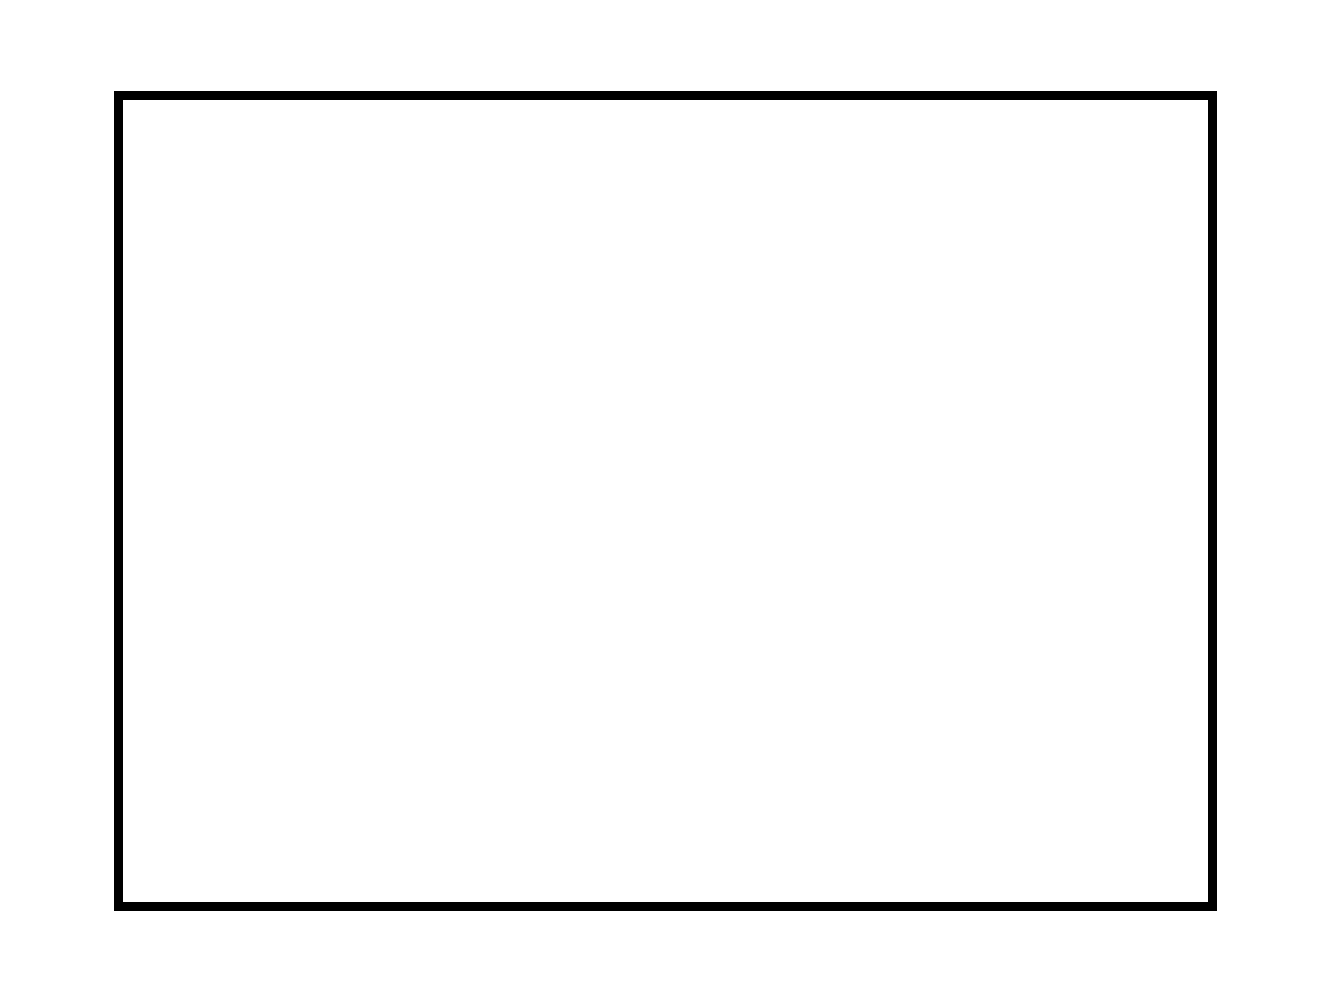
\includegraphics[autoebb, width=200pt]{./img/test.pdf}
    \caption{Datacenter Lane Network Model}
    %\ecaption{The control loop in DCTCP}
    \label{fig:lane_model}
    \end{center}
\end{figure}

\subsection{経路切り替えアルゴリズム}
次に, $\S$\ref{subsec:lane_model}にて示した, データセンターモデルに対して, フローを指向毎に区別,
経路切り替えアルゴリズムを示す.
このアルゴリズムでは, SLに対してより輻輳のない状態に保ち, フロー持続時間の長いものについては, LLに切り替えることで,
それぞれの指向を最大限達成することを実現する. 
先にも述べた通り, 通信経路は送信元アドレスと, 宛先アドレスによって決定され, 基本的にはTCPコネクションを形成する通信経路は同じものになり,
今回想定する環境においても同様である. 
そこでこのアルゴリズムでは, 以下のような動作によって通信の切り替えが行われる. 
\begin{enumerate}
\item SLに対してTCPコネクションを形成する
\item 互いの持つアドレスを交換し合い, サブフローを形成する
\item サブフローを形成した際, 送信元アドレスの$Lane Info$がLLであれば, cwnd=1を代入する. 
\item アルゴリズムがフローをロングフローであると判断すれば,  SLのサブフローに対してcwnd=0を代入し,
LLのサブフローに対して設定されている服装制御のアルゴリズムを適用する
\end{enumerate} 
ここで, 上記のアルゴリズムを実現するための実装上の課題がある. 

\underline{$\cdot$ どのようにフローを区別するのか} \\
先に示した通り, データセンターのアプリケーショントラフィックを考えたときに, それぞれの用途によって指向が異なる. 
既存研究ではフローサイズ($\geq 100KB$)をメトリックとして区別を行っていたが,
現状の実装だとカーネルにおいては通信開始時点でフローサイズがどのくらいになるかは分かり得ない. 
そのため本提案手法では, 主なメトリックとして`` フロー持続時間''を用いる.
これにより, 例えば最も単純な手法においては, フロー持続時間を直接用いて, それを越えた時間通信するフローをレイテンシ指向なロングフロー,
それ以内に完結するフローをショートフローと仮定して制御を行う. 

\underline{$\cdot$ いつ経路を切り替えるのか} \\
フロー持続時間のしきい値を用いた最も単純な手法として, 例えば300[ms]と設定することで,
300[ms]を越えた時点でフローの切り替えが行われるような制御が考えられる. 
しかし, SLが混雑しているにもかかわらず, 持続して通信を行うことや, LLが混雑しているにもかかわらず,
しきい値を超えると経路を切り替える状況も想定されるため, このような単純な手法だと経路の状況に合わせた制御をすることはできない. 
そのため, 経路を切り替えるためのメトリックとして`` リンクコスト''を定義し, コストベースの経路切り替え手法を提案する. 

\subsubsection{コストベースの経路切り替え手法}

提案するコストベースの経路切り替え手法によるトラフィック制御では, スイッチ, エンドノードに対してそれぞれのキューの混雑具合を考慮し, 経路を決定する.
本質的な狙いは, フローサイズに従って通信が終えるということであり, 具体的には,
フローサイズの大きいバックグラウンドフローが通信している中でショートフローが発生した場合,
バックグラウンドフローが占有しているキューを避けた経路で通信することでフロー完結時間を抑えるというシナリオを実現するものである.

\underline{$\cdot$ RTT(Round-Trip Time)$\tau(t)$モデル化} \\
今クライアントノードでのACKパケットを受けた時のRTTを$\tau(t)$とする. 
この時, $d_{l, i}(t)$はリンク$i$におけるリンク伝送遅延, $d_{p, i}(t)$は伝搬遅延, $d_{q,
i}(t)$はキュー遅延を表している. 
この時, エンドノード間の経路として$m$個のネットワーク機器を介する時, 以下のような式でRTTを表現できる. 
\begin{eqnarray}
\tau(t) = \sum ^m _{i=1} \Bigl(d_{l, i}(t) + d_{p, i}(t) + d_{q, i}(t)  \Bigr)
\end{eqnarray}
一般にセッションの間, ネットワーク内の経路は安定して通信を行うと想定することができ, 伝送遅延$d_{l, i}(t)$と伝搬遅延$d_{p,
i}(t)$は定数としてみることができ, それらを併せてRTTに対するバイアスとしてみることができる. 
RTTが変化する最も大きな要因の一つは, 経路ごとのキューイング時間の変化である. 

キューイング時間の変化を最も単純なモデル式で表すと, ノード$i$におけるキュー長$q_i(t)$とリンク容量$c_i$を用いて,
ノード$i$での時間$t_i$での$d_{q,i}(t)$はキュー遅延を以下のように表現することができる. 
\begin{eqnarray}
d_{q,i}(t) = \frac{q_i(t_i)}{c_i}
\end{eqnarray}
これによりACKパケットを受け取った時の時刻$t$におけるRTTは以下のように簡単化される. 
\begin{eqnarray}
\tau(t) = \sum ^m _{i=1} \frac{q_i(t_i)}{c_i} + bias
\end{eqnarray}

\underline{$\cdot$ SL, LLに対するリンクコスト} \\
ここで$\tau_0$は最小RTT, $d_0$は最小キュー遅延を用いて, キューイング遅延の変化量である相対キュー遅延$\nu(t)$を以下のように表す. 
\begin{center}
\begin{eqnarray}
\nu_{i}(t) &=& \tau(t) - \tau_0 \\
&=& \Bigl( \sum ^m _{i=1} \frac{q_i(t_i)}{c_i} + bias \Bigr) - \Bigl( \sum
^n_{i=1} \frac{q'_i(t_i)}{c_i} + bias \Bigr) \\
&=& d_t -d_0
\end{eqnarray}
\end{center}
この$\nu(t)$が通信経路の状況を表すと仮定し,
これをパラメータとしたリンクパフォーマンス関数\cite{bpr}としてリンクコストを以下のように定義する.
リンクコストについては, Davidson関数を参考に導出した\cite{bpr, davidson}.

\begin{eqnarray}
\left\{
\begin{array}{l}
t_{a}^{SL} = t_0 \cdot \bigl\{ 1 + \alpha \cdot \nu(t)^\beta + \tau_0 \bigr\} +
{\rm sgn} (t - t_{deadline}) \cdot \gamma (t - t_{deadline})^\delta \\
t_{a}^{LL} = t_0 \cdot \bigl\{ 1 + \alpha \cdot \nu(t)^\beta + \tau_0 \bigr\} 
\end{array}
\right.
\end{eqnarray} 
ここで, $t^{SL}_a(t), t^{LL}_a(t)$はそれぞれSL, LLのリンクコスト値であり, $t_0$は最小リンクコスト,
$sgn(t)$は符号関数, $t_{deadline}$はしきい値, $\alpha \sim \delta$はパラメータである.
一般に, このリンクコスト関数の変数, パラメータの性質はTable. \ref{table:link_cost_nature}のように表され,
パラメータ$\alpha \sim \delta$については, $\S$\ref{sec:eval}にて検証を行う. 
このリンクパフォーマンス関数を用いた, 通信経路切り替えアルゴリズムをAlgorithm \ref{alg1}に示す. 
このアルゴリズムによって, サブフローが形成された際に, しきい値$t_{deadline}$が設定され(Initialization),
ACKパケットが届き, TCPスタックによるRTTの推定がされた時にコスト計算され(Calculating link-cost),
それぞれのサブフローのリンクコストとの比較を行い(Judging Phase), SLのコストがLLよりも大きくなった場合,
LLの方が有利に通信ができると判断され($judge_flag \Leftarrow 1$), SLのウィンドウサイズを0に,
LLのウィンドウサイズを設定している輻輳制御アルゴリズムに従って算出された値を適用する. 
SLのコストがLLよりも小さいままの場合, SLのウィンドウサイズは服装制御に従い, LLのウィンドウサイズは1に設定される. 
これは, LLの用いる通信経路の状況を把握するため, 非常に小さなパケットを流しRTTを推定するためである. 


\begin{table}[t]
    \begin{center}
    \begin{tabular}{|c|c|}
    \hline
    Variables, Parameter & Nature \\ \hline \hline
    $\alpha$ & \parbox{25zw}{リンクコスト関数の立ち上がりの速さを示す. $\alpha$が小さい場合,
    キューイング遅延の影響が大きくなってもあまりRTTが増加しない }\\ \hline
    $\beta$ & \parbox{25zw}{リンクコスト関数の傾きの度合いを示す.
    経路の通信環境が悪化し$\nu$が大きくなる領域は$\beta$の影響が支配的になる領域である.
    $\beta$が大きいと混雑に対する感度がよりアグレッシブな挙動を示す. } \\ \hline
    $\gamma$ & \parbox{25zw}{しきい値$t_{deadline}$へ近づく速さを示す. $\gamma$が小さい場合,
    しきい値を設定することによるSLの優位性が小さくなる. }\\ \hline
    $\delta$ &
    \parbox{25zw}{リンクコスト関数のしきい値$t_{deadline}$に近づく傾きの度合いを示す.
    $\delta$が大きいとよりしきい値に対する影響が強くなり, 通信状況よりもしきい値に対する挙動の影響が大きくなる. } \\ \hline
    $sgn(t-t_{deadline})$ &
    \parbox{25zw}{リンクコスト関数のしきい値$t_{deadline}$を超えるまでの挙動の違いを示す. しきい値を超えない時間では,
    上に凸の関数をとなり, しきい値を超えると上に凸の挙動を示し, しきい値を超えた時の増加の速さが大きくなり, しきい値に対する影響が大きくなる. }
    \\
    \hline
    \end{tabular}
    \caption{The Natures of the parameter and variables in Link Cost Function}
    \label{table:link_cost_nature}
    \end{center}
\end{table}


\begin{algorithm}
\caption{Caluculating link-cost}
\label{alg1}
\begin{algorithmic}[1]
\STATE $\triangleright $ \underline{Initialzation}
\STATE $t_{deadline} \Leftarrow now + THRESHOLD$
\STATE $\tau_0 \Leftarrow 0$
\STATE $t_{0} \Leftarrow 1$
\STATE $\triangleright $ \underline{Receiving ACK packet:Calculating link-cost}
\STATE $j = $ which subflow the ACK is
\STATE $RTT_j = $ RTT estimation by TCP stack with smoothing
\STATE $measurement\_cost = $ Calculating link-cost
\STATE $cost_j \Leftarrow 3/4  \ast cost_j + 1/4 \ast measurement\_cost$
\COMMENT {Updating cost value with smoothing}
\STATE $base\_RTT = $ Updating if the RTT is the smallest one
\STATE $base\_cost = $ Updating if the cost is the smallest one
\FOR{$i=0$ to $SUBFLOW\_NUMBER$}
\STATE $Min\_Cost's Lane \Leftarrow$ Detecting lane\_info of minimum cost(LL
or SL)
\ENDFOR
\STATE $\triangleright $ \underline{Judging phase}
\IF {$Min\_Cost's Lane$ is LL(Long-flow Lane)}
\STATE $judge\_flag \Leftarrow $ 1
\COMMENT {Change subflow's state}
\ENDIF
\IF {$judge\_flag = 1$}
\STATE {$\triangleright$} \underline{Switching phase}
    \IF {$lane\_info = 1$}
    \STATE $cwnd \Leftarrow 0$
    \COMMENT {This subflow in SL}
    \ELSE
    \STATE $cwnd \Leftarrow $ tcp\_congestion\_control
    \COMMENT {This subflow in LL}
    \ENDIF
\ELSE
\STATE {$\triangleright$} \underline{Keeping state phase}
    \IF {lane\_info = 1}
    \STATE $cwnd \Leftarrow $ tcp\_congestion\_control
    \COMMENT {This subflow in SL}
    \ELSE
    \STATE $cwnd \Leftarrow 1$
    \COMMENT {This very small traffic in LL for probe }
    \ENDIF
\ENDIF
\end{algorithmic}
\end{algorithm}

\section{Discussion}

\subsection{利点}
提案手法は, $\S$\ref{sec:expected_effect}に示す, 性能障害を次のように解決する. \\
{\bf Queue buildup}\\
提案手法では, しきい値, リンクコスト値を用いてロングフローであると判定された場合, 速やかにSLへとトラフィックが移行する. 
これにより, SLはレイテンシ指向なショートフローに対して, 通信経路を良好な状態に保つことができ, FCTを短縮化される. 
また, ロングフローに対しても, ショートフローによって輻輳状態となったLLを避けて通信することができるため, スループットの改善が期待できる. 

しかし実質的には, フローの種類が未知である通信当初については, すべてのフローがSLで通信される. 
このため, ショートフローが短時間に大量に発生した場合や, ロングフローとショートフローが同時に通信を開始した場合には, 通信性能が劣化することが考えられる. 

\subsection{MPTCP実装:IPアドレスペア問題}
現状のMPTCPの実装上, サブフローを形成する際での信負荷の分散が有効に働かない問題がある. 
今, Fig.\ref{fig:mptcp_pair}のような複数インタフェースを持つエンドノード間の通信を考える. 
この時, 現状のMPTCP実装では, 互いのアドレスを交換(ADD\_ADDRESS)しあった後,
フルメッシュな組み合わせのIPアドレスでサブフローが形成される. 
具体的には, 1つのTCPコネクション($F1{src:10.1.0.1, dst:10.2.0.1}$)と3つのサブフロー($F2{src:10.1.0.1,
dst:10.2.1.1}, F3{src:10.1.1.1, dst:10.2.0.1}, F4{src:10.1.1.1,
dst:10.2.1.1}$)が形成される. 
静的なIPベースのルーティングを想定した環境において, フロー$F1$はサーバ側へのデータパケット通信に対して$Data:S1-S2-S4$,
クライアント側へのACKパケット通信に対しては$ACK:S1-S2-S4$の経路をそれぞれ用いる. 
同様に, フロー$F2$は$Data:S1-S2-S4, ACK:S1-S3-S4$, フロー$F3$は, $Data:S1-S3-S4,
ACK:S1-S2-S4$, フロー$F4$は, $Data:S1-S3-S4, ACK:S1-S3-S4$の経路をそれぞれ通る. 
基本的にデータパケット通信の方がデータサイズもパケットの数も多いため, キューイング遅延がより起こりやすい通信であり, 例えばフロー$F1$to
$F2$では異なるサブフローにも関わらず, Dataパケットは同一の経路を通る. 
また, MPTCPはそれぞれのフローを同一のものとして輻輳制御を行うため, 経路によってはトラフィックが偏る可能性があり, 有効的な経路利用を実現できない. 

今回のような複数の経路を持つネットワーク環境において, 通信不可の分散の点から理想的なサブフローの形成は,
1つのTCPコネクション(${src:10.1.0.1, dst:10.2.0.1}$)と1つのサブフロー(${src:10.1.1.1,
dst:10.2.1.1}$)が形成されることである. 
すなわち, 1インタフェース1サブフローの原則による, 重複のないIPアドレスのペアを形成することで, 最適なトラフィック負荷の分散を実現できる. 
そのため, 本提案手法の実装にあたり, 今のMPTCP実装に対して変更を加えた. 


\begin{figure}[t]
    \begin{center}
    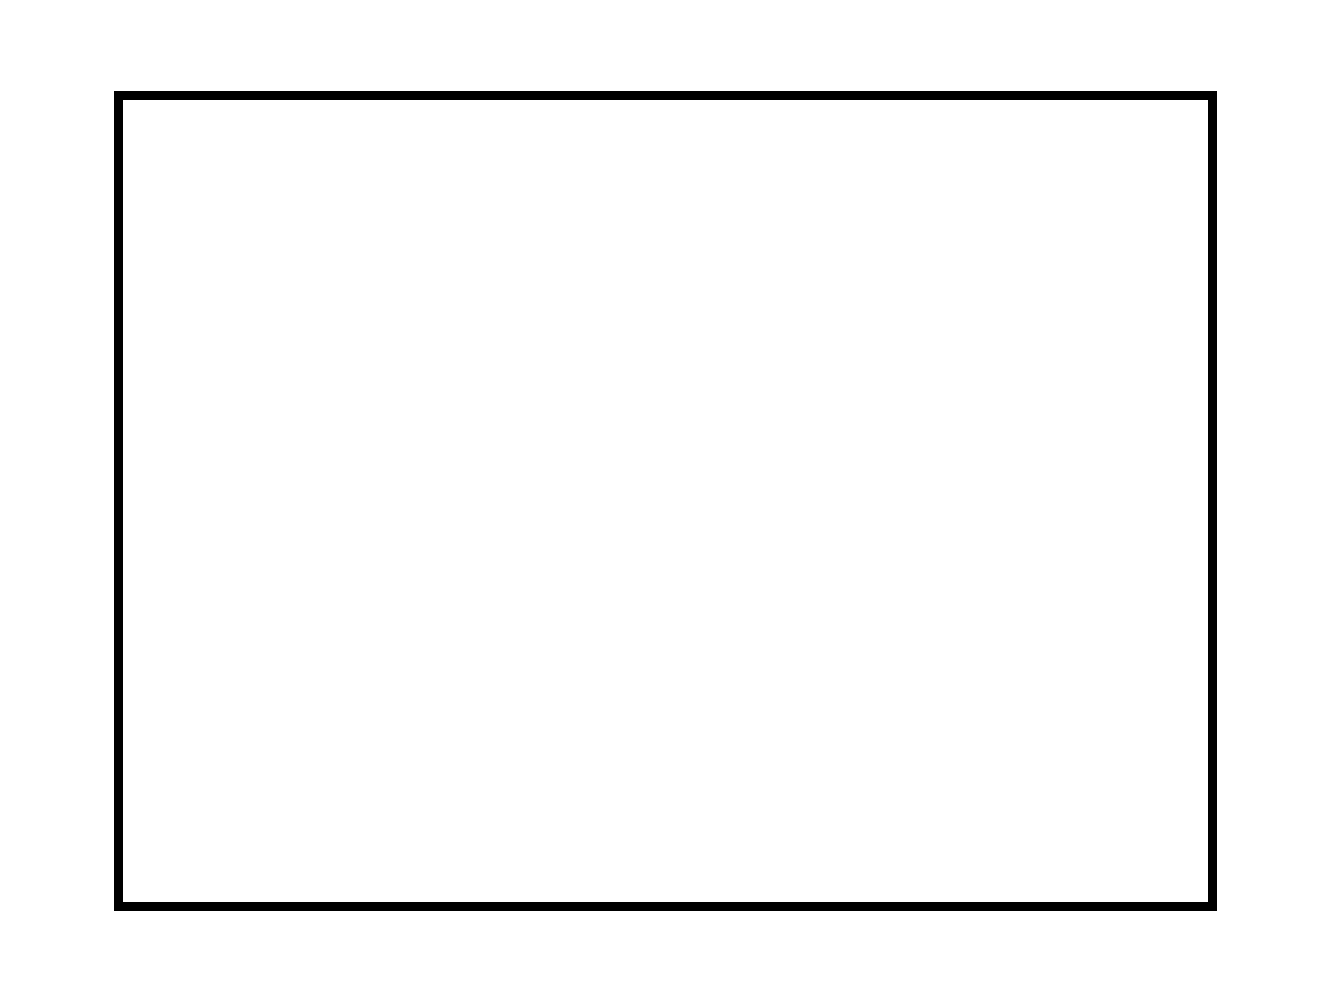
\includegraphics[autoebb, width=200pt]{./img/test.pdf}
    \caption{Techinical problem of creating subflow without complete paired IP
    addressses}
    %\ecaption{The control loop in DCTCP}
    \label{fig:mptcp_pair}
    \end{center}
\end{figure}

\subsection{MHFT形成するためのコスト}
ネットワーク帯域の効率的な利用を目指す取り組みとして, 様々なデータセンターネット枠トポロジーが提案されている. 
提案されているトポロジーは, 複数の等コストな経路がある冗長性を持たせた構成になっており, そうした経路を有効活用する手段としてMPTCPがある. 
$\S$\ref{sec:expected_effect}に示したように, MPTCPを用いることで,
将来の広帯域化により発生すると予想されているノード側のボトルネックについても, 解決することができると期待されている. 
具体的には, 今日のサーバでは一般的である複数のNICに対してMPTCPを利用するということである. 
そこで本研究では, エンドノードの持つ複数のNICを有効活用するためのトポロジーとして, MHFTを提案した. 
しかし, 今日の巨大なクラスターを持つデータセンターの設計には, 性能の優位さだけではなく構築に掛かるコスト二ついても考慮しなければならない. 
そこで, MHFT構築に掛かるコストについて, 保有できるエンドノードの台数とともに検討を行う. 
検討には, エッジ部分でのスイッチとして48ポート1ギガビットスイッチ(\$7000)とアグリゲーション,
コア部分でのスイッチとして128ポート10ギガビットスイッチを用いて構成する際のコストを検討する\cite{fattree}.
なお, 配線ケーブルのコストは考慮しないこととする. 

Fig.\ref{fig:MHFT_cost}に, 保有できるホストの数とトポロジー形成に掛かる費用の関係を示す. 
例えば, 20000ホストに対するスイッチ機器を考えたとき, Fattreeトポロジーでは, 1152台のedgeスイッチ,
1152台のAggregationスイッチ, 576台のcoreスイッチによって構成することができ, かかる費用は約\$1217Mである. 
一方MHFTにおいて20000ホストを保有するトポロジーを構築しようとすると, 

\begin{figure}[t]
    \begin{center}
    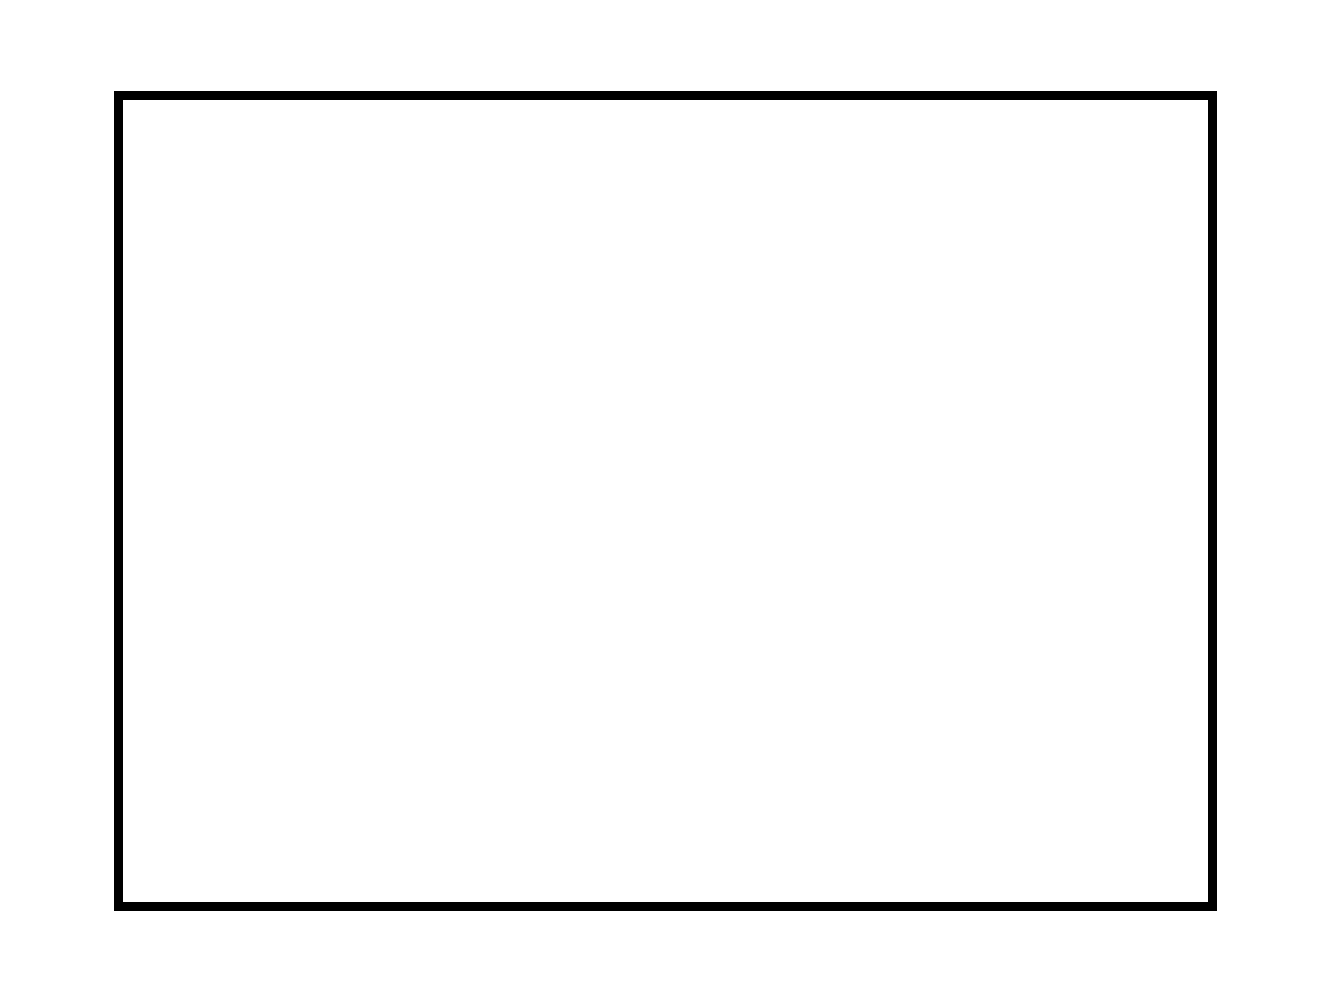
\includegraphics[autoebb, width=200pt]{./img/test.pdf}
    \caption{Current cost estimation vs. maximum possible number of hosts}
    %\ecaption{The control loop in DCTCP}
    \label{fig:MHFT_cost}
    \end{center}
\end{figure}

\subsection{アルゴリズム実装の検討}
提案手法では, 通信可能なすべてのサブフローに対して通信状況を表すリンクコストを計算し, 通信経路を切り替える際のメトリックとして用いる. 
その際, 最も重要な変数の一つはRTTである. 
今回の提案手法では, RTTの推定にはTCPスタックのtcp\_rtt\_estimator用いる.
この推定結果を用いてリンクコストの計算を行うが, RTTや前のパケットの到着時間の差分の揺らぎによっては, リンクコスト値も大きく変動する. 
そのため, リンクコストの平滑化を行う(Line 9). 

また通信開始時のSLでの通信の際にも, LLのリンクコストを計算する必要があるため, LLでのウィンドウサイズを1に設定し,
小さなトラフィックを流す(Line 31).
これにより, すべての経路について経路状況を見ることができ, 経路状況に合わせた制御をすることができる. 





